\chapter{Numerical Optimization and Training of Neural Networks}

\section{Introduction: the Perceptron}

The first model that introduced the idea of a neural network was the perceptron. 
The perceptron is a simple model that takes a set of inputs and produces an output. 
The model is based on the idea of a neuron in the brain, which receives signals from 
other neurons and produces an output signal.\\

The perceptron is a linear model that takes a set of binary inputs 
$x = (x_1, x_2, \ldots, x_n)$ and produces an output $y$ in the following way:

\begin{equation}
    y = \begin{cases}
        1 & \text{if } w_1 x_1 + w_2 x_2 + \ldots + w_n x_n + b > 0\\
        0 & \text{otherwise}
    \end{cases}
\end{equation}

where $w = (w_1, w_2, \ldots, w_n)$ are the weights of the model and $b$ is the bias.
Note that this can be represented as a vector product:

\begin{equation}
    y = \begin{cases}
        1 & \text{if } w \cdot x + b > 0\\
        0 & \text{otherwise}
    \end{cases}
\end{equation}

The perceptron is a simple model that can be used to classify data into two classes.
The model is trained by adjusting the weights and bias to minimize the error on the 
training data.\\

Note that the perceptron is a linear model, which means that it can only learn linearly
separable functions. This means that the model can only learn functions that can be
separated by a hyperplane. If the data is not linearly separable, the perceptron will 
not be able to learn the function.\\

This problem is illustrated by the XOR function, which is not linearly separable.

\subsection{The XOR problem}

The XOR logical function is a simple function that takes two binary inputs and 
produces an output, which is 1 if the inputs are different and 0 if the inputs 
are the same. The XOR function is defined as follows:

\begin{table}[H]
    \centering
    \begin{tabular}{|c|c|c|}
        \hline
        $x_1$ & $x_2$ & $y$\\
        \hline
        0 & 0 & 0\\
        0 & 1 & 1\\
        1 & 0 & 1\\
        1 & 1 & 0\\
        \hline
    \end{tabular}
    \caption{XOR function}
\end{table}

Note that the XOR function is not linearly separable, i.e., it is not possible to
separate the data points with a hyperplane. For instance, the following plot shows
the XOR function in the input space:

\begin{figure}[H]
    \centering
    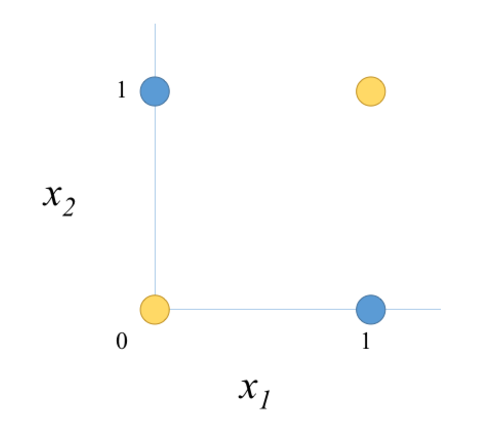
\includegraphics[width=0.5\textwidth]{figures/xor_plot.png}
    \caption{XOR function in the input space}
    \label{fig:xor_plot}
\end{figure}

As we can see, the data points are not linearly separable, which means that 
the perceptron alone cannot learn the XOR function. This is a limitation of
the perceptron model. However, let us take a look at how we can overcome this
limitation by using a more complex model: the multi-layer perceptron.

\subsection{NAND gate}

The NAND gate is a simple logical function that takes two binary inputs and
produces an output, which is 0 if both inputs are 1 and 1 otherwise. The NAND
gate is defined as follows:

\begin{table}[H]
    \centering
    \begin{tabular}{|c|c|c|}
        \hline
        $x_1$ & $x_2$ & $y$\\
        \hline
        0 & 0 & 1\\
        0 & 1 & 1\\
        1 & 0 & 1\\
        1 & 1 & 0\\
        \hline
    \end{tabular}
    \caption{NAND gate}
\end{table}

The NAND gate is an example of a function that is linearly separable, i.e., it can
be separated by a hyperplane. This means that the perceptron can learn the NAND
gate function. Notice that the NAND gate is an universal gate, which means that
it can be used to implement any logical function. This is an important property
of the NAND gate, as it allows us to build more complex functions using simple
building blocks.\\

Because the NAND gate can represent any logical function by combining multiple
gates, and the perceptron can learn the NAND gate, we can use the perceptron to
learn any logical function, just by combining multiple perceptrons. This is the
raw idea behind the multi-layer perceptron.

\subsection{The problem of the step function}

Notice that the perceptron uses a step function to produce the output. It takes 
the value 1 if the input is greater than 0 and 0 otherwise. This has some problems,
as it implies that possible small changes in the input and weights can lead to a
discontinuous change in the output, i.e., big jumps in the output. This can make
the optimization process difficult.\\

To overcome this problem, we can use a different activation functions, such as the
sigmoid function, which is a smooth function that takes values between 0 and 1.
The idea of using a continuous activation function, combined with multiple layers
of perceptrons, is the basis of the multi-layer perceptron.


\section{The Multi-Layer Perceptron}

The multi-layer perceptron (MLP) is a neural network model that consists of multiple
layers of perceptrons. On the output layer, we use a different activation function
than the step function, such as the sigmoid function. This allows the model to learn
more complex functions, as it can approximate any continuous function.\\

We can represent the MLP model using a graph, where each node represents a perceptron
and each edge represents a weight. The graph is organized in layers, where each layer
is connected to the next layer. The input layer represents the input data, the output
layer represents the output of the model, and the hidden layers represent the intermediate
layers of the model.\\

\begin{figure}[H]
    \centering
    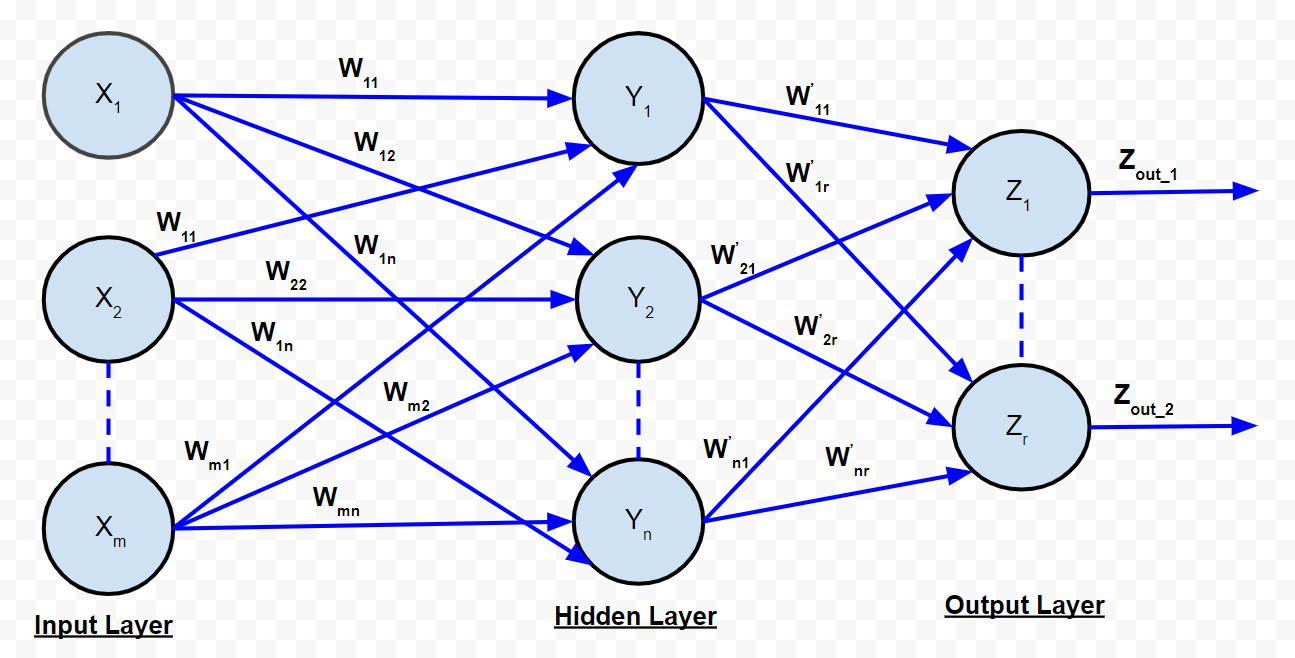
\includegraphics[width=0.7\textwidth]{figures/MLP.jpg}
    \caption{Graph representation of the MLP model}
    \label{fig:mlp_graph}
\end{figure}

For a neuron $j$ in layer $\ell$, we have the following:

\begin{equation}
    z_j^\ell = \sum_{k} w_{jk}^\ell a_k^{\ell-1} + b_j^\ell
\end{equation}

where $z_j^\ell$ is the weighted sum of the inputs of neuron $j$ in layer $\ell$,
$w_{jk}^\ell$ is the weight of the connection between neuron $k$ in layer $\ell-1$
and neuron $j$ in layer $\ell$, $a_k^{\ell-1}$ is the output after activation
of neuron $k$ in layer $\ell-1$, and $b_j^\ell$ is the bias of neuron $j$ in 
layer $\ell$.\\

Notice that in each output layer, we apply an activation function to the weighted sum
of the inputs. This activation function is a non-linear function that allows the model
to learn complex functions. This is represented by:

\begin{equation}
    a_j^\ell = \sigma(z_j^\ell)
\end{equation}

where $\sigma$ is the activation function. In general, we can represent the weights
as a matrix $W^\ell$ and the biases as a vector $b^\ell$. This allows us to write
the equation that represents the output of a particular layer as follows:

\begin{equation}
    a^\ell = \sigma(W^\ell a^{\ell-1} + b^\ell)
\end{equation}
    
where $a^\ell$ is the output of layer $\ell$, $a^{\ell-1}$ is the output of layer
$\ell-1$, and $\sigma$ is the activation function. This equation represents the
forward pass of the model, i.e., the process of computing the output of the model
given an input.\\

Now, on the output layer, we need a function that can represent the distance between
the output of the model and the true output. This function is called the loss function,
and it measures the error of the model. The main goal of training a neural network is
to minimize the loss function.

\section{Training a Neural Network}

To train a neural network, we need to define a loss function that measures the error
of the model. This function takes the
output of the model and the true output and produces a value that represents how
well the model is performing. In general, a loss function $J$ should have the 
following properties:

\begin{enumerate}
    \item $J$ can be written as an average of the loss over the training data.
    $$J = \frac{1}{N} \sum_{i=1}^{N} J_s$$
    where $N$ is the number of samples in the training data and $J_s$ is the loss
    for sample $s$.

    \item $J$ is a function only of the output of the model and the true output.
\end{enumerate}

Now, to train the model, we need to minimize the loss function. This is done by
adjusting the weights and biases of the model to reduce the error. This process
is called optimization. There are many optimization algorithms that can be used
to train a neural network, but in general, all of them follow the same idea:
compute the gradient of the loss function with respect to the weights and biases
and update the weights and biases in the opposite direction of the gradient.
This is called gradient descent.\\

Therefore, our aim is to compute the derivative of the loss function with respect
to the weights and biases of the model, i.e., we need to compute:

\begin{equation}
    \frac{\partial J}{\partial k^\ell_{jk}}, \frac{\partial J}{\partial b^\ell_j} \quad \forall \ell, j, k
\end{equation}

where $k^\ell_{jk}$ is the weight of the connection between neuron $k$ in layer $\ell-1$
and neuron $j$ in layer $\ell$, and $b^\ell_j$ is the bias of neuron $j$ in layer $\ell$.\\

For this, let us define the vector of errors (or sensitivities) $\delta^\ell$ for 
layer $\ell$ as follows:

\begin{equation}
    \delta^\ell_j = \frac{\partial J}{\partial z^\ell_j} \quad \forall j
\end{equation}

where $z^\ell_j$ is the weighted sum of the inputs of neuron $j$ in layer $\ell$.
The vector of errors $\delta^\ell$ represents how much the error changes with respect
to the weighted sum of the inputs of neuron $j$ in layer $\ell$.\\

Now, we will deduce 4 funcamental equations that will allow us to compute the
gradient of the loss function with respect to the weights and biases of the model.
These equations are called the backpropagation equations, and they are the key
to training a neural network.\\

\subsection{Backpropagation equations}

\begin{enumerate}
    \item Compute the error of the output layer $\delta^L$:
    
    $$\delta^L_j = \frac{\partial J}{\partial z^L_j} = \sum_{k} \frac{\partial J}{\partial a^L_k} \cdot \frac{\partial a^L_k}{\partial z^L_j} $$
    
    Because $a^L_k$ only depends on $z^L_k$ if $k = j$, we have:

    $$\delta^L_j = \frac{\partial J}{\partial a^L_j} \cdot \frac{\partial a^L_j}{\partial z^L_j}$$
    
    Notice that:
    $$\frac{\partial a^L_j}{\partial z^L_j} = \sigma'(z^L_j)$$ 
     
    where $\sigma'$ is the derivative of the activation function. Then, we have:

    $$\delta^L_j = \frac{\partial J}{\partial a^L_j} \cdot \sigma'(z^L_j)$$

    Notice that the value of $z^L_j$ has already been computed in the forward pass.
    Rewriting the equation in vector form, we have:

    \begin{equation}
        \delta^L = \nabla_{a^L} J \odot \sigma'(z^L)
    \end{equation}

    where $\nabla_a J$ is the gradient of the loss function with respect to the output
    of the model and $\odot$ is the element-wise product.

    \item Compute the error of the hidden layers $\delta^\ell$ with respect to $\delta^{\ell+1}$:
    
    $$\delta^\ell_j = \frac{\partial J}{\partial z^\ell_j} = \sum_{k} \frac{\partial J}{\partial z^{\ell+1}_k} \cdot \frac{\partial z^{\ell+1}_k}{\partial z^\ell_j}$$

    Notice that: 
    
    $$\frac{\partial J}{\partial z^{\ell+1}_k} = \delta^{\ell+1}_k$$

    Then, we have:

    $$\delta^\ell_j = \sum_{k} \delta^{\ell+1}_k \cdot \frac{\partial z^{\ell+1}_k}{\partial z^\ell_j}$$

    Now, we need to compute the derivative of $z^{\ell+1}_k$ with respect to $z^\ell_j$.
    Notice that:

    $$z^{\ell+1}_k = \sum_{m} w^{\ell+1}_{km} a^\ell_m + b^{\ell+1}_k  = \sum_{m} w^{\ell+1}_{km} \sigma(z^\ell_m) + b^{\ell+1}_k$$

    Then, we have:

    $$\frac{\partial z^{\ell+1}_k}{\partial z^\ell_j} = w^{\ell+1}_{kj} \cdot \sigma'(z^\ell_j)$$

    Finally, we have:

    $$\delta^\ell_j = \sum_{k} \delta^{\ell+1}_k \cdot w^{\ell+1}_{kj} \cdot \sigma'(z^\ell_j)$$

    Rewriting the equation in vector form, we have:

    \begin{equation}
        \delta^\ell = ((W^{\ell+1})^T \delta^{\ell+1}) \odot \sigma'(z^\ell)
    \end{equation}

    \item Compute the gradient of the loss function with respect to $b^\ell$:
    
    $$\frac{\partial J}{\partial b^\ell_j} = \frac{\partial J}{\partial z^\ell_j} \cdot \frac{\partial z^\ell_j}{\partial b^\ell_j}$$

    Notice that:

    $$z_j^\ell = \sum_{k} w_{jk}^\ell a_k^{\ell-1} + b_j^\ell$$

    Then, we have:

    $$\frac{\partial z^\ell_j}{\partial b^\ell_j} = 1$$

    Finally, we have:

    $$\frac{\partial J}{\partial b^\ell_j} = \delta^\ell_j$$

    Rewriting the equation in vector form, we have:

    \begin{equation}
        \nabla_{b^\ell} J = \delta^\ell
    \end{equation}

    \item Compute the gradient of the loss function with respect to $W^\ell$:
    
    $$\frac{\partial J}{\partial w^\ell_{jk}} = \frac{\partial J}{\partial z^\ell_j} \cdot \frac{\partial z^\ell_j}{\partial w^\ell_{jk}}$$

    Notice that:

    $$z_j^\ell = \sum_{k} w_{jk}^\ell a_k^{\ell-1} + b_j^\ell$$

    Then, we have:

    $$\frac{\partial z^\ell_j}{\partial w^\ell_{jk}} = a_k^{\ell-1}$$

    Finally, we have:

    $$\frac{\partial J}{\partial w^\ell_{jk}} = \delta^\ell_j \cdot a_k^{\ell-1}$$

    Rewriting the equation in matrix form, we have:

    \begin{equation}
        \nabla_{W^\ell} J = \delta^\ell (a^{\ell-1})^T
    \end{equation}

\end{enumerate}

These are the backpropagation equations, which allow us to compute the gradient of the
loss function with respect to the weights and biases of the model. This is the key to
training a neural network. By computing the gradient of the loss function and updating
the weights and biases in the opposite direction of the gradient, we can minimize the
error of the model and learn complex functions.\\

Summarizing the equations:

\begin{enumerate}
    \item Compute the error of the output layer:
    $$\delta^L = \nabla_{a^L} J \odot \sigma'(z^L)$$

    \item Compute the error of the hidden layers:
    $$\delta^\ell = ((W^{\ell+1})^T \delta^{\ell+1}) \odot \sigma'(z^\ell)$$

    \item Compute the gradient of the loss function with respect to $b^\ell$:
    $$\nabla_{b^\ell} J = \delta^\ell$$

    \item Compute the gradient of the loss function with respect to $W^\ell$:
    $$\nabla_{W^\ell} J = \delta^\ell (a^{\ell-1})^T$$
\end{enumerate}

Then, the backpropagation algorithm can be summarized as follows:

\begin{enumerate}
    \item $x$ is the input to the model. Compute $a^1$
    \item For each layer $\ell$ from $2$ to $L$:
    \begin{enumerate}
        \item Compute $z^\ell = W^\ell a^{\ell-1} + b^\ell$
        \item Compute $a^\ell = \sigma(z^\ell)$
    \end{enumerate}
    \item Compute the loss function $J$
    \item Compute the error of the output layer $\delta^L$
    \item For each layer $\ell$ from $L-1$ to $1$:
    \begin{enumerate}
        \item Compute the error of the hidden layers $\delta^\ell$
        \item Compute the gradient of the loss function with respect to $b^\ell$
        \item Compute the gradient of the loss function with respect to $W^\ell$
        \item Update the weights and biases:
        \begin{itemize}
            \item $W^\ell = W^\ell - \alpha \nabla_{W^\ell} J$
            \item $b^\ell = b^\ell - \alpha \nabla_{b^\ell} J$
        \end{itemize}

        where $\alpha$ is the learning rate.
    \end{enumerate}
\end{enumerate}

\section{Activation functions}

The activation function of a neuron is a non-linear function that takes the weighted
sum of the inputs of the neuron and produces an output. The activation function is
a key component of a neural network, as it allows the model to learn complex functions.
There are many activation functions that can be used in a neural network, but some
of the most common are:

\begin{enumerate}
    \item Sigmoid function:
    \begin{equation}
        \sigma(z) = \frac{1}{1 + e^{-z}}
    \end{equation}

    The sigmoid function takes values between 0 and 1, which makes it useful for
    binary classification problems. However, the sigmoid function has some problems,
    such as the vanishing gradient problem, which can make training difficult.

    \item Hyperbolic tangent function:
    \begin{equation}
        \tanh(z) = \frac{e^z - e^{-z}}{e^z + e^{-z}}
    \end{equation}

    The hyperbolic tangent function is similar to the sigmoid function, but it takes
    values between -1 and 1. This can make training easier, as the output is centered
    around 0. However, the hyperbolic tangent function also has the vanishing gradient
    problem.

    \item Rectified Linear Unit (ReLU) function:
    \begin{equation}
        \text{ReLU}(z) = \max(0, z)
    \end{equation}

    The ReLU function is a simple function that takes the maximum between 0 and the
    input. The ReLU function is widely used in practice, as it is simple and efficient.
    However, the ReLU function has some problems, such as the dying ReLU problem, which
    can make some neurons inactive.

    \item Leaky ReLU function:
    \begin{equation}
        \text{Leaky ReLU}(z) = \begin{cases}
            z & \text{if } z > 0\\
            \alpha z & \text{otherwise}
        \end{cases}
    \end{equation}

    The Leaky ReLU function is a variant of the ReLU function that allows a small
    gradient when the input is negative. This can help to overcome the dying ReLU
    problem.

    \item Swish function (Google):
    \begin{equation}
        \text{swish}(z) = \frac{z}{1 - e^{-z}}
    \end{equation}

    The swish function is a new activation function that has been proposed recently.
    The swish function is similar to the sigmoid function, but it has a different
    shape that can make training easier. The swish function has been shown to perform
    well on a variety of tasks.

    \item Softmax function:
    \begin{equation}
        \text{softmax}(z)_i = \frac{e^{z_i}}{\sum_{j} e^{z_j}}
    \end{equation}

    The softmax function is a generalization of the sigmoid function that takes a
    vector of inputs and produces a vector of outputs that sum to 1. The softmax
    function is often used in the output layer of a neural network to produce
    probabilities for a classification problem. The softmax function is useful
    when the output of the model needs to be interpreted as a probability distribution.

\end{enumerate}

\section{Loss functions}

The loss function of a neural network is a function that measures the error of the
model. The loss function takes the output of the model and the true output and
produces a value that represents how well the model is performing. There are many
loss functions that can be used in a neural network, but some of the most common
are:

\begin{enumerate}
    \item Mean Squared Error (MSE):
    \begin{equation}
        J = \frac{1}{2N} \sum_{i=1}^{N} (y_i - \hat{y}_i)^2
    \end{equation}

    The mean squared error (MSE) is a simple loss function that measures the squared
    difference between the output of the model and the true output. The MSE is often
    used in regression problems, where the output of the model is a continuous value.

    \item Mean Absolute Error (MAE):
    \begin{equation}
        J = \frac{1}{N} \sum_{i=1}^{N} |y_i - \hat{y}_i|
    \end{equation}

    The mean absolute error (MAE) is a loss function that measures the absolute
    difference between the output of the model and the true output. The MAE is often
    used in regression problems, where the output of the model is a continuous value.

\end{enumerate}

An issue of the MSE is that it can be sensitive to outliers. The MAE is more
robust to outliers, but it can be harder to optimize. In practice, the choice of
loss function depends on the problem at hand.\\

Another big issue of using the MSE is that it can lead to the vanishing gradient
problem. This is because when we derive the MSE with respect to the weights and
biases, we get an expression that depends on the derivative of the activation
function. If the activation function is the sigmoid function, the derivative
of the activation function can be very small, which can make the optimization
process difficult.\\

To overcome this problem, we can use the cross-entropy loss function.

\subsection{Cross-entropy loss function}

The cross-entropy loss function is a loss function that measures the error of the
model by comparing the output of the model with the true output. The cross-entropy
loss function is often used in classification problems, where the output of the
model is a probability distribution. The cross-entropy loss function is defined as
follows:

\begin{equation}
    J = -\frac{1}{N} \sum_{i=1}^{N} \sum_{j} y_{ij} \log(\hat{y}_{ij})
\end{equation}

where $y_{ij}$ is the true output of class $j$ for sample $i$ and $\hat{y}_{ij}$
is the predicted output of class $j$ for sample $i$.\\ 

Let us see why the cross-entropy loss function is useful for avoiding the vanishing
gradient problem. For this, let us take a simple binary classification problem,
with the following loss function:

\begin{equation}
    J = -\frac{1}{N} \sum_{i=1}^{N} y_i \log(\hat{y}_i) + (1 - y_i) \log(1 - \hat{y}_i)
\end{equation}

where $y_i$ is the true output for sample $i$ and $\hat{y}_i$ is the predicted
output for sample $i$.\\

Now, let us compute the derivative of the loss function with respect to one
of the weights of the model. For this, we have:

$$ \frac{\partial J}{\partial w} = \frac{\partial J}{\partial \hat{y}} \cdot \frac{\partial \hat{y}}{\partial z} \cdot \frac{\partial z}{\partial w}$$
    
where $z$ is the weighted sum of the inputs of the neuron and $\hat{y}$ is the
output of the neuron after activation. So we have:

$$ \frac{\partial J}{\partial w} = \frac{\partial J}{\partial \hat{y}} \cdot \sigma'(z) \cdot x$$

where $x$ is the input of the neuron. Now, let us compute the derivative of the
loss function with respect to the output of the neuron:

$$ \frac{\partial J}{\partial \hat{y}} = -\frac{1}{N} \sum_{i=1}^{N} \left( \frac{y_i}{\hat{y}_i} - \frac{1 - y_i}{1 - \hat{y}_i} \right)$$

Notice that we can rewrite $\hat{y}_i$ as $\sigma(z_i)$, where $z_i$ is the weighted
sum of the inputs of the neuron. Then, simplifying, we have:

$$ \frac{\partial J}{\partial \hat{y}} = -\frac{1}{N} \sum_{i=1}^{N} \frac{\sigma(z_i) - y_i}{\sigma(z_i) (1 - \sigma(z_i))}$$

Combining the terms, and using the fact that $\sigma'(z) = \sigma(z) (1 - \sigma(z))$ 
for the sigmoid, we have:

$$ \frac{\partial J}{\partial w} = -\frac{1}{N} \sum_{i=1}^{N} (\sigma(z_i) - y_i) \cdot x$$

This is the gradient of the loss function with respect to the weights of the model.
Notice that the gradient depends on the difference between the output of the model
and the true output. This is the key to avoiding the vanishing gradient problem.\\

The cross-entropy loss function is a generalization of the binary classification
loss function to multi-class classification problems. It avoids the vanishing
gradient problem when using the softmax activation function in the output layer,
which is the generalization of the sigmoid function to multi-class classification.\\

How do we obtain the cross-entropy loss function? Let us derive it.\\

\subsection{Derivation of the cross-entropy loss function}

The idea is to avoid the vanishing gradient problem by letting the derivative
of the loss function to not depend on the derivative of the activation function.
In other terms, we want that these terms:

$$\frac{\partial J}{\partial w} = (a - y) \sigma'(z) x , \quad \frac{\partial J}{\partial b} = (a - y) \sigma'(z)$$

do not depend on $\sigma'(z)$, i.e., we want that:

\begin{equation}
    \frac{\partial J}{\partial w} = (a - y) x , \quad \frac{\partial J}{\partial b} = (a - y)
\end{equation}

where $a$ is the output of the neuron after activation, $y$ is the true output, $z$
is the weighted sum of the inputs of the neuron, $w$ is the weight of the connection
between the neuron and the previous layer, and $b$ is the bias of the neuron.\\

Let us take the derivative with respect to the bias $b$, and notice the following:

$$\frac{\partial J}{\partial b} = \frac{\partial J}{\partial a} \cdot \frac{\partial a}{\partial z}$$
$$ = \frac{\partial J}{\partial a} \cdot \sigma'(z) = \frac{\partial J}{\partial a} \cdot a (1 - a)$$

Now, we want that this term does not depend on $\sigma'(z)$, and for that, we 
use the equation (3.22):

$$\frac{\partial J}{\partial a} a (1 - a) = a - y$$

Then, we have:

$$\frac{\partial J}{\partial a} = \frac{a - y}{a (1 - a)}$$

Integrating, we obtain:

$$J = - ( y \log(a) + (1 - y) \log(1 - a)) + C$$

which is the cross-entropy loss function.\\

\section{Regularization}

Regularization is a technique used to prevent overfitting in a neural network.
Overfitting occurs when the model learns the training data too well and fails
to generalize to new data. Regularization is a way to prevent overfitting by
adding a penalty term to the loss function. This penalty term discourages the
model from learning complex functions that fit the training data too well.\\

There are many regularization techniques that can be used in a neural network,
but some of the most common are:

\begin{enumerate}
    \item \textbf{L2 regularization:}
    \begin{equation}
        J = J_0 + \lambda \frac{1}{2 N} \sum_{\ell} \sum_{j, k} (w^\ell_{jk})^2
    \end{equation}

    L2 regularization is a technique that adds a penalty term to the loss function
    that is proportional to the square of the weights of the model. L2 regularization
    encourages the model to learn small weights, which can help to prevent overfitting
    by reducing the complexity of the model.\\

    Notice that, when computing the update of the weights, we have:

    $$w^{(k + 1)} = w^{(k)} - \alpha \nabla_{w^{(k)}} J = w^{(k)} - \alpha \nabla_{w^{(k)}} J_0 - \alpha \frac{\lambda}{N} w^{(k)}$$

    which is equivalent to:

    $$w^{(k + 1)} = (1 - \alpha \frac{\lambda}{N}) w^{(k)} - \alpha \nabla_{w^{(k)}} J_0$$

    When choosing appropiate values for $\lambda$, notice that the term $\alpha \frac{\lambda}{N} < 1$.
    This causes the weights to decay over time, which can help to prevent overfitting. This is 
    called weight decaying.\\

    \item \textbf{L1 regularization:}
    \begin{equation}
        J = J_0 + \lambda \frac{1}{N} \sum_{\ell} \sum_{j} |w^\ell_j|
    \end{equation}

    L1 regularization is a technique that adds a penalty term to the loss function
    that is proportional to the absolute value of the weights of the model. L1
    regularization encourages the model to learn sparse weights, i.e., weights
    that are close to zero. This can help to prevent overfitting by reducing the
    complexity of the model.\\

    Notice that, when computing the update of the weights, we have:

    $$w^{(k + 1)} = w^{(k)} - \alpha \nabla_{w^{(k)}} J = w^{(k)} - \alpha \nabla_{w^{(k)}} J_0 - \alpha \frac{\lambda}{N} \text{sign}(w^{(k)})$$

    This means that the weights are updated by subtracting (or adding) a constant value from
    the weights. This can help to prevent overfitting by encouraging the model to learn
    sparse weights.\\


    \item \textbf{Dropout regularization:}
    
    Dropout regularization is a technique that randomly sets a fraction of the
    neurons in the model to zero during training. This can help to prevent
    overfitting by reducing the complexity of the model. Dropout regularization
    is a simple and effective technique that can be used in a variety of models.\\

    The idea is, for some layer $\ell$, to set a fraction $p$ of the neurons to zero.
    This can be done by multiplying the output of the layer by a mask $m$ that has
    values of 0 or 1. The mask $m$ is generated by sampling from a Bernoulli distribution
    with probability $p$. Then, the output of the layer is given by:

    $$a^\ell = m \odot \sigma(z^\ell)$$

    where $\odot$ is the element-wise product. This can help to prevent overfitting
    by reducing the complexity of the model.

    \begin{figure}[H]
        \centering
        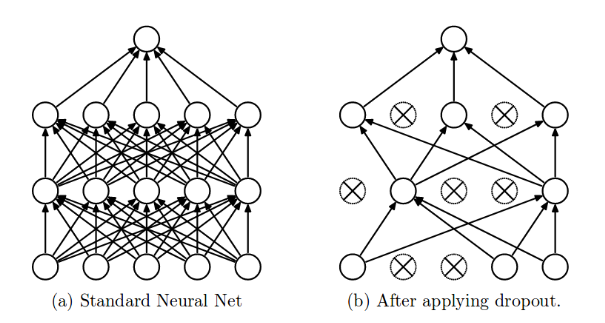
\includegraphics[width=0.7\textwidth]{figures/dropout.png}
        \caption{Dropout regularization}
        \label{fig:dropout}
    \end{figure}

\end{enumerate}








